% ordinal-networks: software paper. Target: Chaos (AIP), regular Article.
% Build: pdflatex manuscript && bibtex manuscript && pdflatex manuscript && pdflatex manuscript
% Every measured number comes from numbers.tex, which is written by make_numbers.py from
% results/*.json; every figure is written by make_figures.py. Do not type numbers by hand.
\documentclass[aip,cha,reprint,amsmath,amssymb]{revtex4-2}
\usepackage{graphicx}
\usepackage{booktabs}
\usepackage{hyperref}
\usepackage[T1]{fontenc}
\usepackage{upquote}
% Generated by paper/make_numbers.py from paper/results/*.json. Do not edit.
\newcommand{\nCores}{16}
\newcommand{\machine}{Windows-11-10.0.26300-SP0}
\newcommand{\pyVersion}{3.14.7}
\newcommand{\ordpyVersion}{1.2.3}
\newcommand{\nOrdpyMax}{10^{7}}
\newcommand{\speedupN}{870}
\newcommand{\tOnEight}{0.85}
\newcommand{\tMmax}{0.53}
\newcommand{\tOrdpyMthree}{3.1}
\newcommand{\tOrdpyMlast}{80}
\newcommand{\mOrdpyLast}{25}
\newcommand{\scaleSix}{4.8}
\newcommand{\scaleSixteen}{2.4}
\newcommand{\mEntropy}{16}
\newcommand{\errTPE}{19}
\newcommand{\errG}{7.6}
\newcommand{\errRho}{0.2}
\newcommand{\tSweepLog}{5.5}
\newcommand{\tQuick}{0.23}
\newcommand{\maxDiffH}{0}
\newcommand{\maxDiffC}{0}
\newcommand{\scaleExp}{8}
\newcommand{\scaleMmax}{22}
\newcommand{\scaleRho}{0.6163}
\newcommand{\scaleSeconds}{89}
\newcommand{\scaleEigMinutes}{34}
\newcommand{\scaleNodes}{1.6}
\newcommand{\scaleAgreeM}{8}
\newcommand{\scaleRhoPrev}{0.5649}
\newcommand{\scaleShortCross}{16}
\newcommand{\scaleShortLast}{0.20}
\newcommand{\collapseN}{15\,479\,530}
\newcommand{\collapsePEbefore}{0.832}
\newcommand{\collapsePEafter}{0.715}
\newcommand{\collapseRho}{0.688}
\newcommand{\collapseNmax}{2\times10^{7}}


\newcommand{\pkg}{\texttt{ordinal-networks}}
\newcommand{\code}[1]{\texttt{#1}}
\newcommand{\TODO}[1]{\textbf{[TODO: #1]}}

\begin{document}

\title{ordinal-networks: fast ordinal symbolisation and ordinal partition networks for very long time series}

\author{Konstantinos Sakellariou}
\email{\TODO{corresponding e-mail}}
\affiliation{\TODO{affiliation}}
% \TODO{co-authors: decide with T. Stemler and M. Small}

\date{\today}

\begin{abstract}
Ordinal methods turn a time series into a sequence of permutations and study the
frequencies of these patterns and of the transitions between them. Their estimates of
dynamical invariants converge slowly in the pattern length $m$, and the number of
possible patterns grows as $m!$, so informative results need long patterns and long
series. Existing open-source tools materialise every window in memory and are practical
only for short patterns. We present \pkg{}, a Python library with a multi-core Rust
core that symbolises series of up to $10^9$ points with pattern lengths up to $m = 34$,
streaming the input from disk and the results to disk when they exceed memory. Each
pattern receives a fixed, decodable integer identifier, its lexicographic rank among all
$m!$ permutations, so results are comparable across series and no pattern dictionary is
stored. On top of the symbolisation the library implements ordinal partition networks as
Markov models of the dynamics: four estimators of topological entropy, an ordinal
estimate of the sum of positive Lyapunov exponents, entropy rate, cycle detection,
network measures and surrogates by random walk. On a \nCores-thread laptop, $10^{8}$
points are symbolised at $m = 6$ in \tOnEight~s, \speedupN{} times faster than the
reference Python implementation at the largest size the latter completes. Where the two
implementations overlap they agree to machine precision. The library is MIT-licensed and
every figure in this paper is regenerated by one script.
\end{abstract}

\maketitle

\begin{quotation}
Replacing the values of a time series by their order relations gives a description of
the dynamics that is robust to noise and to monotone distortions of the measurement, and
that needs no choice of partition. The price is combinatorial: there are $m!$ possible
patterns of length $m$, and quantities such as the topological entropy are approached
only as $m$ grows. In practice this has confined ordinal analysis to short patterns,
where the estimates are far from converged. This paper describes software that removes
the computational limit, so that the convergence can be observed rather than assumed.
\end{quotation}

\section{Introduction}

Bandt and Pompe~\cite{bandt2002} proposed to characterise a time series by the relative
frequencies of the order patterns of $m$ consecutive values. The resulting permutation
entropy, the count of forbidden patterns, and the complexity--entropy
plane~\cite{lamberti2004,rosso2007} are now standard tools of nonlinear time-series
analysis. Ordinal partition networks~\cite{small2013,mccullough2015} add the temporal
order of the patterns: nodes are the observed patterns and directed, weighted edges count
the transitions between consecutive windows. Read as a Markov chain on the ordinal
partition, such a network is a finite-state model of the dynamics~\cite{sakellariou2019},
from which invariants such as the topological entropy can be estimated through the
spectrum of its connectivity matrix~\cite{sakellariou2021}.

These estimates share a practical difficulty. For interval maps the growth rate of the
number of admissible patterns equals the topological entropy~\cite{bandt2002b}, but the
limit in $m$ is approached slowly, and resolving patterns of length $m$ needs series
much longer than the number of admissible patterns. Useful results therefore need both
large $m$ and large $N$.

Open-source software for ordinal analysis has grown considerably. The \code{ordpy}
package~\cite{pessa2021} covers the breadth of Bandt--Pompe methods, including
two-dimensional data and ordinal networks~\cite{pessa2019}; \code{pyunicorn}~\cite{donges2015}
provides recurrence and visibility networks. These tools build an array of all windows
in memory and identify patterns by sorting and comparing rows. This is simple and
adequate for short patterns, but time and memory grow quickly with $N$ and $m$
(Sec.~\ref{sec:performance}).

\pkg{} is built for the complementary regime. Its contributions are:
\begin{enumerate}
\item \emph{Scale.} Series of $10^9$ points and patterns up to $m = 34$, with
multi-core counting, memory-mapped input and out-of-core results.
\item \emph{Ordinal partition networks as Markov models.} Topological-entropy
estimators, the ordinal Lyapunov sum, entropy rate, cycles, network measures and
surrogates, in one object.
\item \emph{Fixed, decodable pattern identifiers}, comparable across series, chunks
and parameter values.
\end{enumerate}
It does not aim at the breadth of \code{ordpy}: two-dimensional data and
amplitude-aware variants are out of scope. Table~\ref{tab:compare} states the overlap,
and Sec.~\ref{sec:validation} shows that the overlapping quantities agree.

The library is installed with \code{pip install ordinal-networks}; prebuilt wheels
need no compiler. Source, documentation and the scripts that regenerate every figure
of this paper are at \url{https://github.com/k-sakel/ordinal-networks}
(\TODO{Zenodo DOI of the tagged release}).

\begin{table}
\caption{\label{tab:compare}Scope of \pkg{} (version 0.2.0) and \code{ordpy}
(version \ordpyVersion). \TODO{extend with antropy, EntropyHub, pyunicorn, teaspoon and
ComplexityMeasures.jl once benchmarked on the same hardware.}}
\begin{ruledtabular}
\begin{tabular}{lcc}
 & \pkg{} & \code{ordpy} \\
\hline
Pattern distribution, permutation entropy & yes & yes \\
R\'enyi and Tsallis entropies & yes & yes \\
Complexity--entropy plane & yes & yes \\
Ordinal network, global node entropy & yes & yes \\
Missing patterns and transitions & yes & yes \\
Two-dimensional data & no & yes \\
Weighted / amplitude-aware entropies & no & yes \\
Topological entropy estimators & yes & no \\
Ordinal Lyapunov sum, entropy rate & yes & no \\
Cycle detection, network measures & yes & no \\
Surrogates by random walk & yes & no \\
Maximum pattern length & 34 & memory-bound \\
Out-of-core input and results & yes & no \\
Multi-core & yes & no \\
\end{tabular}
\end{ruledtabular}
\end{table}

\section{Quick start}

\begin{verbatim}
>>> import ordinal_networks as on
>>> x = on.systems.generate("logistic",
...         "ChaosR4", n=10**7)
>>> stats = on.OrdinalSymbolizer(m=12).fit(x)
>>> stats.n_patterns, stats.n_transitions
(10525, 21001)
>>> net = stats.network()
>>> net.spectral_radius(log=True)
0.6920
>>> net.lyapunov_sum()
0.6872
\end{verbatim}
Both values estimate $\ln 2 = 0.6931$, the topological entropy and the Lyapunov
exponent of the fully chaotic logistic map (outputs rounded to four digits). The
symbolisation of the $10^7$ points takes \tQuick~s on the machine of
Sec.~\ref{sec:performance}.

\section{Ordinal symbolisation at scale}

\subsection{Definitions}

A series $x_0, \dots, x_{N-1}$ is cut into windows of $m$ points with embedding delay
$\tau$ and slide $w$: window $k$ holds $x_{kw + j\tau}$, $j = 0, \dots, m-1$, and there
are $\lfloor (N - (m-1)\tau - 1)/w \rfloor + 1$ windows. The default $w = 1$ gives
maximally overlapping windows; $w = m\tau$ gives disjoint ones.

A window is mapped to a permutation in one of two equivalent conventions. The
\emph{chronological} ranking~\cite{bandt2002} lists the time indices in order of
increasing value, $\pi = (p_1, \dots, p_m)$ with $x_{p_1} < \dots < x_{p_m}$. The
\emph{amplitude} ranking~\cite{small2013} gives each point, in time order, its rank in
decreasing amplitude. Equal values are ordered by time, the earlier point counting as
smaller~\cite{bandt2002}; the number of windows with ties is reported, so that the user
can judge whether quantisation matters. Windows containing NaN or $\pm\infty$ are
skipped, and no transition is recorded into or out of a skipped window, so the chain is
never joined across a gap.

\subsection{Fixed pattern identifiers}

Each pattern is identified by its 1-based lexicographic rank among the $m!$
permutations of $(1, \dots, m)$. With $c_k$ the number of entries to the right of
position $k$ that are smaller than $\pi_k$ (the Lehmer code),
\begin{equation}
\mathrm{id}(\pi) = 1 + \sum_{k=1}^{m} c_k\,(m-k)! .
\end{equation}
The identifier is computed in $O(m)$ with a bit mask and a population count, and is
exact in 128-bit integers up to $m = 34$ ($34! < 2^{128}$). It depends only on the
pattern, not on the data set, so identifiers are comparable across series, across the
chunks and threads of one computation, and across runs; and it is invertible, so no
dictionary of patterns is stored:
\begin{verbatim}
>>> on.encode([3, 1, 2])
5
>>> on.decode(5, 3)
array([3, 1, 2], dtype=uint8)
>>> on.pattern_of([0.3, 0.9, 0.1])
5
\end{verbatim}

\subsection{Algorithm}

The pipeline has four stages.

\emph{Streaming.} The input is read in chunks of a fixed number of windows from a
memory-mapped file, so memory use is independent of $N$.

\emph{Incremental ranking.} Each chunk is divided among threads. A thread keeps the
rank vector of the current window. When consecutive windows overlap, the oldest point
is removed and the newest inserted by comparing it with the $m-1$ retained points, at
$O(m)$ cost per window instead of a sort; tie counts are updated in the same pass. The
rank vector is converted to the identifier through its Lehmer code.

\emph{Counting.} Patterns and transitions (pairs of consecutive identifiers) are
counted in per-thread hash tables that are merged after each chunk. A transition across
a chunk or thread boundary is counted by carrying the last identifier forward.

\emph{Spill and merge.} When the tables exceed a memory budget they are sorted and
written to disk as runs; at the end the runs are combined by a $k$-way merge. For large
$m$ and $N$, where almost every window is a new pattern, the result itself can be
streamed to memory-mapped files instead of being assembled in memory.

The pattern and transition counts are identical for every chunk size, thread count
and memory budget; the test suite asserts this. Several pattern lengths can be
processed in one pass over the data (\code{sweep}).

\begin{verbatim}
>>> sym = on.OrdinalSymbolizer(m=25,
...     memory_budget=3 * 2**30)
>>> stats = sym.fit("henon_x.npy",
...     output="HENON_m25")
>>> sweep = sym.sweep("henon_x.npy",
...     m=range(2, 23))
\end{verbatim}

Results are stored as two Parquet tables, the pattern frequencies and the transition
edge list, which together define the Markov chain.

\section{Ordinal statistics}

From the pattern frequencies $p_i$ the library computes the permutation
entropy~\cite{bandt2002}, R\'enyi and Tsallis entropies, the fraction of forbidden
patterns, and the Jensen--Shannon statistical complexity~\cite{lamberti2004,rosso2007}
$C = Q_J[P, U]\,H[P]$, where $H$ is the normalised permutation entropy, $U$ the uniform
distribution on all $m!$ patterns and $Q_J$ the normalised Jensen--Shannon divergence.
The $m! - V$ unobserved patterns contribute to $Q_J$ through a closed-form term, so $C$
is evaluated for any $m \le 34$ without enumerating permutations.

From the transition counts $w_{ij}$ it computes the conditional entropy of the next
pattern given the current one, the global node entropy~\cite{mccullough2017,pessa2019}
and the fraction of missing transitions. The conditional entropy uses the source
marginal $p_i = \sum_j w_{ij} / \sum_{kl} w_{kl}$ rather than the pattern frequency; the
two differ because the last window of every uninterrupted run has no successor, and
only the former gives a non-negative quantity for short or gapped series.

\begin{verbatim}
>>> st = on.OrdinalSymbolizer(m=6).fit(x)
>>> st.permutation_entropy(normalized=True)
>>> st.complexity_entropy()      # (H, C)
>>> st.conditional_entropy()     # bits
>>> st.forbidden_fraction()
\end{verbatim}

\subsection{Validation}\label{sec:validation}

Figure~\ref{fig:agreement} reproduces two classic results: the permutation entropy
along the bifurcation diagram of the logistic map~\cite{bandt2002} and the
complexity--entropy plane~\cite{rosso2007}. Values computed with \code{ordpy} are
overlaid; over the points compared the two packages return identical floating-point
values (largest absolute difference \maxDiffH{} in $H$ and \maxDiffC{} in $C$). The test suite extends this comparison to pattern
distributions, R\'enyi and Tsallis entropies, missing patterns and links, global node
entropy and the full weighted edge list of the network, for four series and pattern
lengths 3 to 6, and requires equality to $10^{-12}$ or exact equality of counts.

\begin{figure*}
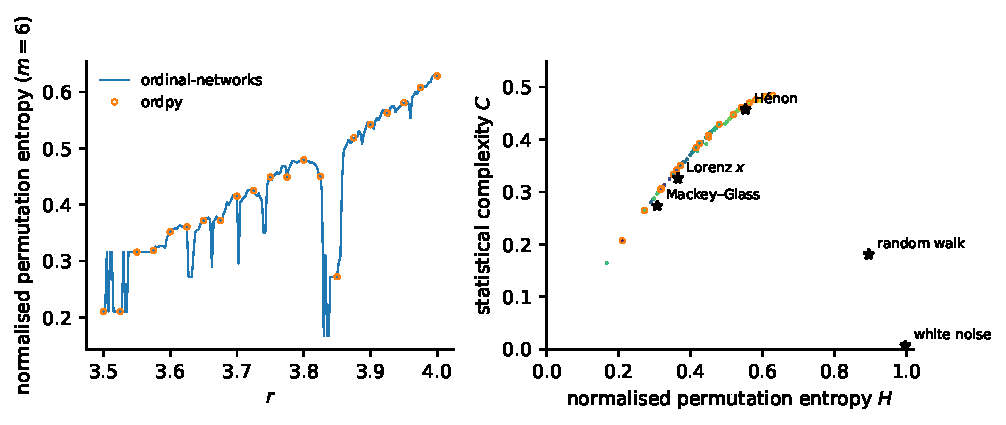
\includegraphics[width=0.8\textwidth]{figures/agreement_ordpy}
\caption{\label{fig:agreement}Agreement with \code{ordpy}. Left: normalised
permutation entropy ($m = 6$) of the logistic map against $r$; circles are
\code{ordpy} values. Right: complexity--entropy plane for the same orbits (colour: $r$)
and for five reference series (stars). Regenerate with
\code{paper/make\_figures.py --only agreement}.}
\end{figure*}

\section{Ordinal partition networks as Markov chains}

The network of a symbolised series is obtained with \code{stats.network()}. Let
$W_{ij}$ be the number of transitions from pattern $i$ to pattern $j$, $A$ the binary
matrix with $A_{ij} = 1$ where $W_{ij} > 0$, $T$ the row-stochastic matrix
$T_{ij} = W_{ij}/\sum_k W_{ik}$ and $Q$ the column-normalised matrix
$Q_{ij} = W_{ij}/\sum_k W_{kj}$. All are available as sparse matrices.

\subsection{Topological entropy}

Four estimators are implemented~\cite{sakellariou2021}, with $V(m)$ the number of
observed patterns: (I) the slope of $\ln V(m)$ against $m$; (II) the topological
permutation entropy $\ln V(m)/(m-1)$~\cite{bandt2002b}; (III) $\ln G(m)$, where $G$ is
the mean number of admissible $(m+1)$-patterns that extend an admissible $m$-pattern;
and (IV) $\ln \rho(A)$, the logarithm of the spectral radius of the connectivity matrix.
\begin{verbatim}
>>> sweep = on.OrdinalSymbolizer(2).sweep(
...     x, range(2, 22))
>>> on.entropy.entropy_table(sweep,
...     lyapunov=True)
\end{verbatim}
Figure~\ref{fig:entropy} shows them for the logistic map at $r = 4$, where the exact
value is $\ln 2$. Methods I--III approach it from above and are still
\errTPE\% (II) and \errG\% (III) too high at $m = \mEntropy$; Method IV is within
\errRho\% at $m = 12$. Beyond $m \approx 15$ the estimates of Method IV and of the
Lyapunov sum turn down, the signature of undersampling at this series length
(Sec.~\ref{sec:scale}).

\begin{figure}
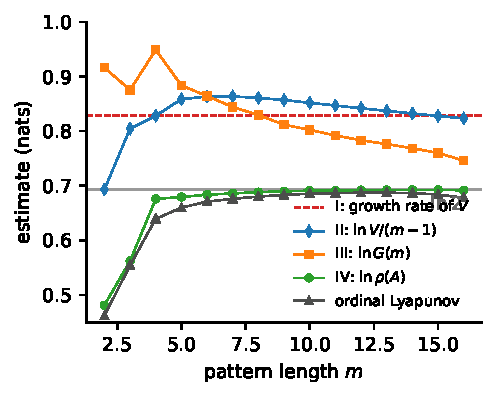
\includegraphics[width=\columnwidth]{figures/entropy_logistic}
\caption{\label{fig:entropy}Estimators of the topological entropy of the logistic map
($r = 4$, $N = 10^7$), and the ordinal Lyapunov estimate, against pattern length. All
pattern lengths were symbolised in one pass in \tSweepLog~s.}
\end{figure}

\subsection{Ergodic quantities}

The stationary distribution $\pi$ is the left Perron vector of $T$, and the entropy
rate of the chain is $-\sum_i \pi_i \sum_j T_{ij} \ln T_{ij}$. The ordinal Lyapunov
sum~\cite{sakellariou2019} estimates the sum of positive Lyapunov exponents from $Q$:
with $u$ the leading right eigenvector of $Q$ and $P = \mathrm{diag}(u)^{-1} Q\,
\mathrm{diag}(u)$, which is row-stochastic with stationary vector $v$,
\begin{equation}
\Lambda = -\sum_{ij} v_i P_{ij} \ln Q_{ij} .
\end{equation}
Networks of up to 1500 nodes are treated with a dense eigensolver and larger ones with
ARPACK started from a fixed vector, so results are reproducible.

\subsection{Structure, cycles and surrogates}

Degree and strength sequences, node-link entropy, clustering, assortativity, shortest
paths, centralities and community detection are available as methods; conversion to
\code{igraph} and \code{networkx} objects is provided. The diagonal of $A^k$ identifies
nodes on closed walks of length $k$, and, with the stored symbol sequence, the windows
of the series that lie near unstable periodic orbits of period $k$. A random walk on the
network is a sequence of overlapping patterns; \code{surrogates.reconstruct} turns it
into a series by drawing, for each new pattern, an observed value that satisfies the
order constraint relative to the previous $m - 1$ points.

\section{Performance}\label{sec:performance}

All timings are from one machine: \machine{}, \nCores{} logical processors, 15~GB of
memory, Python~\pyVersion. The task is the same for both packages: from a series in
memory to the pattern distribution and the weighted transition list, for the $x$
component of the H\'enon map, $\tau = 1$, overlapping windows. Each time is the best of
three runs. For \code{ordpy} the task is \code{ordinal\_distribution} followed by
\code{ordinal\_network}.

Figure~\ref{fig:benchmark} gives the results. At $m = 6$ \pkg{} is \speedupN{} times
faster at $N = \nOrdpyMax$, the largest series \code{ordpy} completed within the time
budget, and processes $10^8$ points in \tOnEight~s. At $N = 10^6$ its time is nearly
flat in $m$ up to $m \approx 12$ and \tMmax~s at $m = 34$, while that of \code{ordpy}
rises from \tOrdpyMthree~s at $m = 3$ to \tOrdpyMlast~s at $m = \mOrdpyLast$. With
\nCores{} threads the speed-up over one thread is \scaleSix{} at $m = 6$ and
\scaleSixteen{} at $m = 16$: scaling saturates at about four threads. Encoding is
parallel, but reading the input, counting non-finite values and merging the per-thread
tables are sequential; we have not yet profiled how the remaining time divides between
these stages and memory bandwidth. \TODO{profile before submission.}

\begin{figure*}
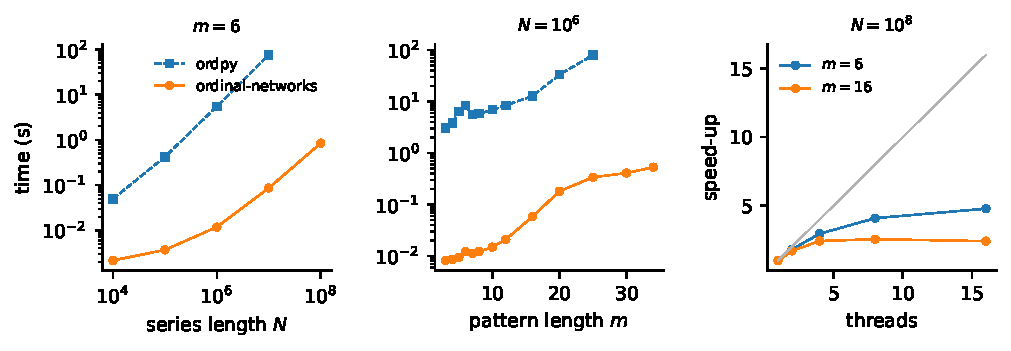
\includegraphics[width=0.85\textwidth]{figures/benchmark}
\caption{\label{fig:benchmark}Time to obtain pattern frequencies and network edge
weights for the H\'enon map. Left: against series length at $m = 6$. Centre: against
pattern length at $N = 10^6$. Right: speed-up against number of threads. Regenerate
with \code{benchmarks/compare.py}.}
\end{figure*}

\TODO{Repeat on a second machine and add peak memory; the repository README reports
$N = 10^9$, $m = 25$ in 242~s on a 2-core, 7~GB virtual machine, measured with version
0.1.0.}

\section{What scale buys}\label{sec:scale}

\subsection{Convergence of the entropy estimate}

Figure~\ref{fig:scale} shows $\ln\rho(A)$ for the H\'enon map ($a = 1.4$, $b = 0.3$)
for series of $10^5$ to $10^{\scaleExp}$ points and $m$ up to \scaleMmax. The
reference value of the topological entropy is $0.4651$~\cite{newhouse1993}. The
estimate decreases with $m$ for every series length, but how fast depends on $N$. For
$N = 10^5$ it passes through the reference value at $m = \scaleShortCross$ and
continues down to \scaleShortLast{} at $m = \scaleMmax$: the network is undersampled,
transitions that exist are not observed, and the agreement with the reference at one
pattern length is coincidental. Each tenfold increase of $N$ lifts the curve at large
$m$. The two longest series agree to within 1\% only up to $m = \scaleAgreeM$; at
$m = \scaleMmax$ the estimates are \scaleRhoPrev{} for $N = 10^{7}$ and \scaleRho{} for
$N = 10^{\scaleExp}$, the latter still well above the reference and still decreasing.

Two conclusions follow. First, for this system the spectral estimate has not converged
at $m = \scaleMmax$ even with $10^{\scaleExp}$ points, so reported agreements obtained
at a single $(N, m)$ should be read with care; convergence has to be judged from
independence of $N$, which requires sweeps of this size. Second, such sweeps are now
cheap on the symbolic side: all pattern lengths $m = 2, \dots, \scaleMmax$ at
$N = 10^{\scaleExp}$ were symbolised in one pass in \scaleSeconds~s. The cost has moved
to the eigenvalue problem, which took \scaleEigMinutes~minutes for the same sweep, the
largest network having $\scaleNodes \times 10^{6}$ nodes.

\begin{figure*}
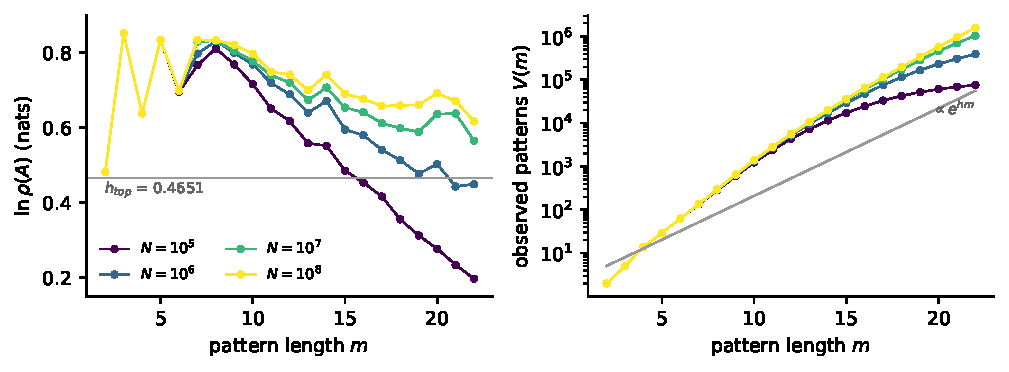
\includegraphics[width=0.8\textwidth]{figures/scale_henon}
\caption{\label{fig:scale}H\'enon map. Left: $\ln\rho(A)$ against pattern length for
increasing series length; the line marks the reference topological
entropy~\cite{newhouse1993}. Right: number of observed patterns; the grey line has
slope $h_{top}$.}
\end{figure*}

\subsection{A caution on long floating-point orbits}

In double precision the orbit of the logistic map at $r = 4$ from $x_0 = 0.4$ lands
exactly on the fixed point $x = 0$ after \collapseN{} stored iterates (following $10^4$
discarded ones), and is constant thereafter (Fig.~\ref{fig:collapse}). A longer series
is increasingly made of tied windows that all carry the same pattern: at $m = 8$ the
permutation-entropy rate $H/(m-1)$ falls from \collapsePEbefore{} to \collapsePEafter{}
nats when the series is extended to $\collapseNmax$ points. The spectral estimate is
unaffected, $\ln\rho(A) = \collapseRho$ throughout, because the constant tail adds a
single self-loop to the network; frequency-based and connectivity-based quantities
differ in their sensitivity to such artefacts. The generators of the library warn when
a trajectory collapses, and the count of tied windows exposes it in any data. Series
much longer than $10^7$ should come from systems whose finite-precision orbits stay
aperiodic for longer, such as the H\'enon map used above, for which no tied window
occurs in $10^{\scaleExp}$ points.

\begin{figure*}
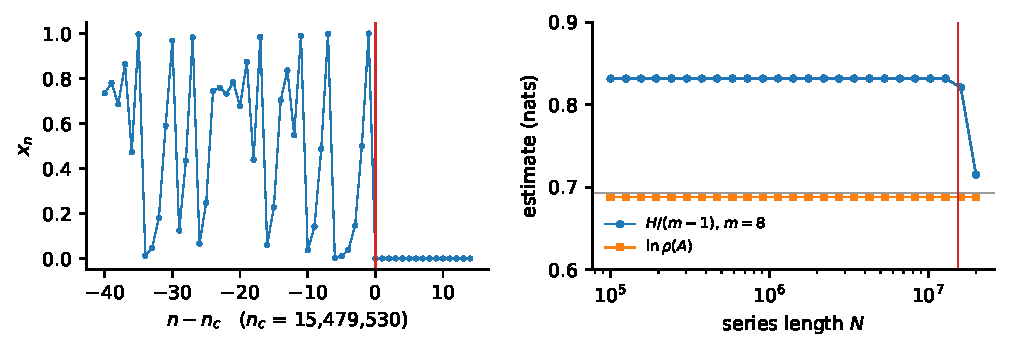
\includegraphics[width=0.8\textwidth]{figures/collapse_logistic}
\caption{\label{fig:collapse}Floating-point collapse of the logistic orbit ($r = 4$).
Left: the orbit around the collapse index $n_c$. Right: permutation-entropy rate and
$\ln\rho(A)$ ($m = 8$) against the length of the analysed series; the vertical line
marks $n_c$.}
\end{figure*}

\section{Real-data case study}

\TODO{One long experimental series end to end, including surrogate testing. The data
set is to be chosen by the authors (candidates: a long PhysioNet ECG/EEG record, a laser
intensity series, a climate record). No results are reported here yet.}

\section{Design notes and limitations}

\emph{Scope.} One-dimensional series only. Amplitude-aware variants (weighted
permutation entropy and relatives) are not implemented.

\emph{Network measures at scale.} Symbolisation scales to networks of $10^7$ nodes and
more; spectral quantities are computed with sparse iterative solvers and remain
practical to about $10^6$ nodes, while path-based measures build dense distance
matrices and are limited to about $10^4$ nodes.

\emph{Parallel scaling.} As shown in Sec.~\ref{sec:performance}, speed-up saturates at
a few threads. Parallelising the merge of the counting tables is the main planned
improvement.

\emph{Flows.} The built-in generators integrate flows with a fixed-step fourth-order
Runge--Kutta scheme, which is adequate for generating test series but not a substitute
for an adaptive integrator.

\emph{Relation to the MATLAB toolbox.} The library ports the code used in
Refs.~\onlinecite{sakellariou2019,sakellariou2021}. Differences, including corrected
errors, are listed in the documentation.

\section{Conclusions}

\pkg{} makes ordinal symbolisation and ordinal partition networks practical for series
and pattern lengths at which the convergence of ordinal estimators can be examined
directly. Fixed pattern identifiers make results comparable and storable without
dictionaries, and the network object gathers the Markov-chain quantities that have so
far been available only in unpublished code.

\begin{acknowledgments}
\TODO{funding and acknowledgments.} \TODO{Disclosure required by the journal: an AI
coding assistant (Claude, Anthropic) was used in developing and reviewing the software
and in drafting this manuscript; the authors reviewed and are responsible for all
content.}
\end{acknowledgments}

\section*{Data availability}

The software, the scripts that generate all series, figures and numbers in this paper,
and the benchmark harness are openly available at
\url{https://github.com/k-sakel/ordinal-networks}, version 0.2.0
(\TODO{Zenodo DOI}). No experimental data were used.

\bibliography{references}

\end{document}
